\chapter{Implementation Details}
This chapter provides a more in-depth explanation of how the different functionalities have been implemented. The main operations that have been added to the L1 API for managing the PUFs are the following:
\begin{itemize}
	\item Fill the host DB with a number of responses received from the device
 	\item Challenge the device and determine the authenticity of such device  
\end{itemize}

To perform these actions correctly, it is necessary to establish a communication between the host and the device (also referred to as \emph{board}). 

The board is responsible for
\begin{enumerate}
	\item Reading the PUF responses from the RAM and store them in the flash;
	\item Providing the list of all PUF responses to the host;
	\item Returning a specific response corresponding to the challenge sent by the host.
\end{enumerate}

On the other hand, the host is in charge of
\begin{enumerate}
	\item Retrieving the list of PUF responses and storing them in a database;
	\item Sending a challenge to the board, retrieving the corresponding response and then comparing it with the one stored in the database.
\end{enumerate}


\section {PUF retrieval and DB initialization}
Before the PUFs can be retrieved, it is necessary to perform a memory erase: this guarantees that the whole PUFs retrieval process starts from a clean state and that the RAM cells assume their stable states at start up.

Then, when the board is powered on, it is necessary to access the SRAM as soon as possible to avoid compromising its content and to copy the values found in the SRAM to the flash memory so that they can be read later on. To perform this operation, tasks on both the host and board side have to be carried out.



\subsection{Host side}

To retrieve the correct data from the RAM (whose values are the PUFs needed to implement the whole authentication mechanism), it is necessary to access the memory immediately after the board's startup and before writing any data in the RAM. 

Once this is done, the host works in three steps. The first one is to prepare the parameters to be send to the board, the second one is to get the response from the board and the last one is to access the DB to store them. All these steps are implemented in the $examples > puf\_db\_init.cpp$ file.

In order to request the PUFs, no parameters need to be sent. In fact, only the whole list of PUFs provided from the board is expected. So, only a variable to store the board response is needed.
The actual communication with the board is done through the use of functions implemented in the L1\_security API. There we added the $L1GetPUFS$ function (see Figure \ref{fig:L1GetPUFS}), which is responsible for transmitting the parameters to the board and receiving the results from it.

\begin{figure}[h!]
	\vspace{0.5cm}
	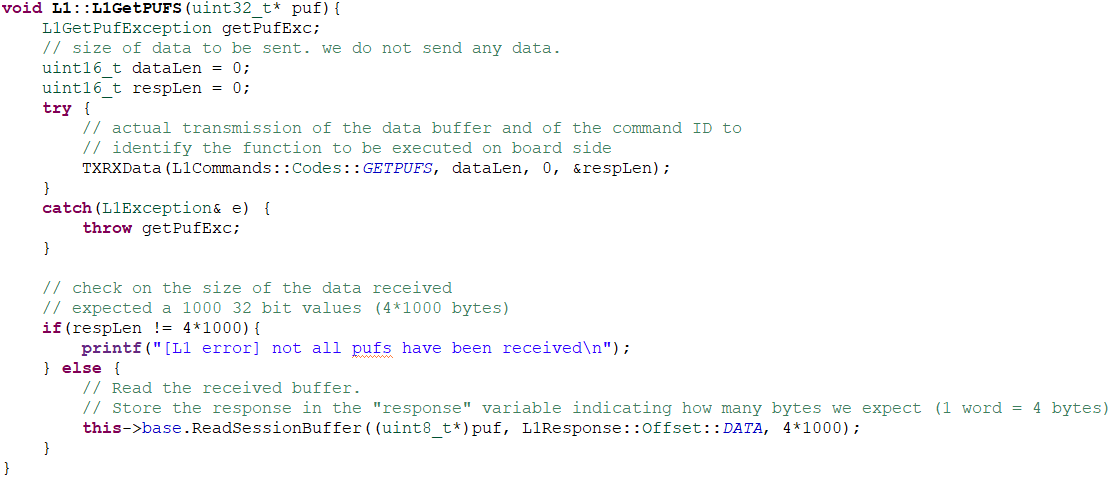
\includegraphics[width = 0.8\textwidth]{images/L1GetPUFS.png}
	\caption{Function responsible for communicating with the board and receiving the list of PUFs. }
	\label{fig:L1GetPUFS}
\end{figure}

As shown in the code in Figure \ref{fig:L1GetPUFS}, 1000 PUFs are expected. The communication between host and board is done through the use of buffers that will then be transmitted using an appropriate transmit/receive function. In the buffer, the data to be sent and the size of the data being transmitted or received need to be set. This buffer is then sent with the command ID of the operation that must be performed on the board side. The response will be transmitted again through a buffer that will store the indicated expected bytes in the indicated variable. After that, the host is responsible for managing that data, which in this case is to write them in a DB.

\subsection{Board side}

In this stage the board is responsible for retrieving the initial data, the PUFs, from the SRAM and store them in the flash memory so that they can be safely accessed later.

Since the content of the RAM will be overwritten, the PUFs must be copied as soon as possible. For this reason, this operation has to be done before any memory initialization. This operation is therefore done in the startup assembly file in which the reset handler can be found. In this way, it is guaranteed that the RAM is read before spoiling its content with other code which would mean compromising the PUFs.

Since the flash needs control registers to be set in order to be accessed in a safe way, we relied on the HAL functions provided by STMicroelectronics. More precisely, the functions to unlock and program/write in memory. The code written to perform this operation can be found in Figure \ref{fig:code_assembly}

\begin{figure}[h!]
	\centering
	\vspace{0.5cm}
	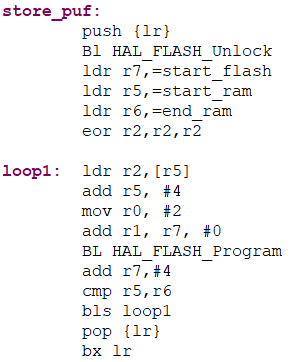
\includegraphics[width = 0.3\textwidth]{images/code_assembly.png}
	\caption{Assembly code to store PUFs into the flash memory. }
	\label{fig:code_assembly}
\end{figure}

As indicated in the reference manual for the MCU STM32F429\cite{STM32F429}, the memory mapping of the SRAM is 0x020000000 -  0x02002FFFF, and 0x08000000 - 0x081FFFFF for the flash memory. The SRAM is therefore scanned in that range of addresses and the retrieved content is then loaded in a section of the flash memory that is not used by the board for its normal functioning.

At the end of the execution of the assembly code, the 1000 expected PUFs are stored in the flash memory which will be accessible once entered in the $main.cpp$ and in the execution loop. 

Once the PUFs are in memory, it is necessary to access them. This is done in the $puf\_retreive()$ function that can be found in the $se3\_dispatcher\_core.c$ file. This is the function associated to the command code transmitted from the host side to the board.

To make the command call possible, it is necessary to define these commands in the $se3\_dispatcher\_core.h$ which must reflect the ID associated to the same command found on the host side.

\begin{figure}[h!]
	\vspace{0.5cm}
	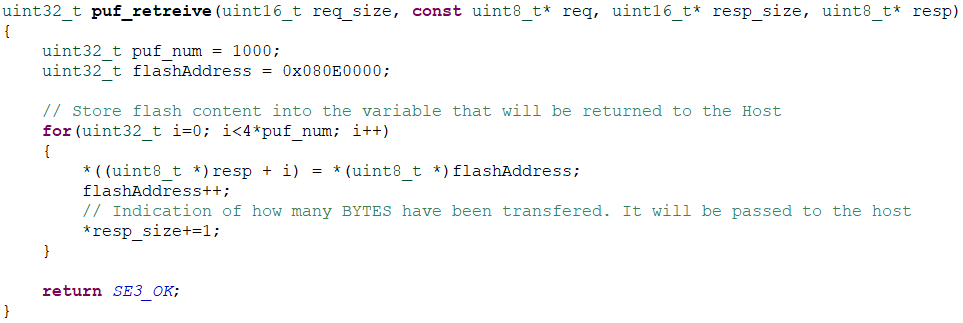
\includegraphics[width = 0.8\textwidth]{images/puf_retreive.png}
	\caption{puf\_retreive function. }
	\label{fig:puf_retreive}
\end{figure}

In the $puf\_retreive()$ function we simply read from the flash the PUFs that we stored at startup. This is the data that will be sent to the host side.


\section {Application of a challenge and verification of the device} 
\label{section:impl_host}

Once we have the DB filled with PUFs, it can be used to check the authenticity of the board by comparing the PUFs in the DB to the ones provided by the board. Again, to implement this functionality, some tasks on both host and board side must be performed.

\subsection{Host side}

The approach is similar to the one used for reading the PUFs, but in this case different parameters must be transmitted. In fact, the challenge needs to be sent to the board. The host is therefore responsible for getting the challenge, using it to access the DB and retrieving the expected response. Then the challenge is sent to the board and the corresponding response is expected in return.

The next step is to perform the actual transmit/receive, which is done using the L1ChallengePUF function of the L1 API (see figure \ref{fig:L1ChallengePUF}).

\begin{figure}[h!]
	\vspace{0.5cm}
	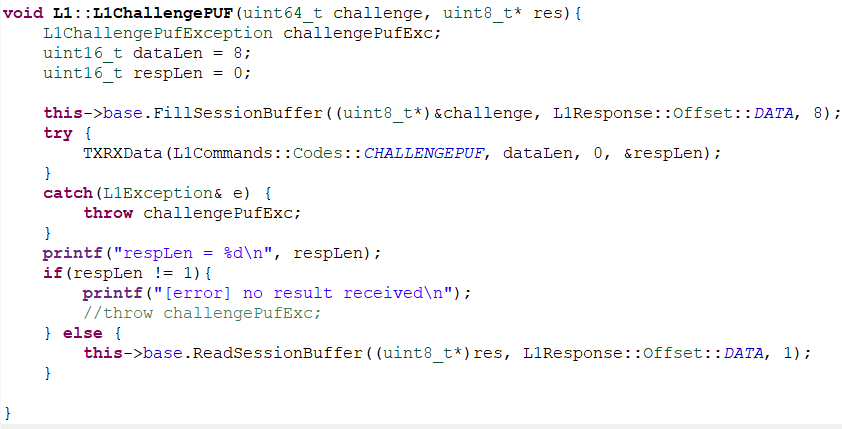
\includegraphics[width = 0.8\textwidth]{images/L1ChallengePUF.png}
	\caption{L1ChallengePUF function for transmitting challenge and response PUF}
	\label{fig:L1ChallengePUF}
\end{figure}


In this function, some data must be transmitted. Because the TXRX works with bytes, it is necessary to provide the size of the data to be sent/received in bytes. This size is equal to 4, since the transmitted challenge is 32bit long. As a response, 32 bits are also expected, hence again 4 bytes.

Once the host has received the response, it compares it with the value corresponding to that challenge that has been previously store in the DB. This comparison is done using a hamming distance. The chosen distance is of 4 bits. This choice is based on statistical results that have been obtained, trading off accuracy and safety. These operations are done in the $examples > puf\_challenge.cpp$ file shown in Figure \ref{fig:puf_challenge.cpp}

\begin{figure}[h!]
	\vspace{0.5cm}
	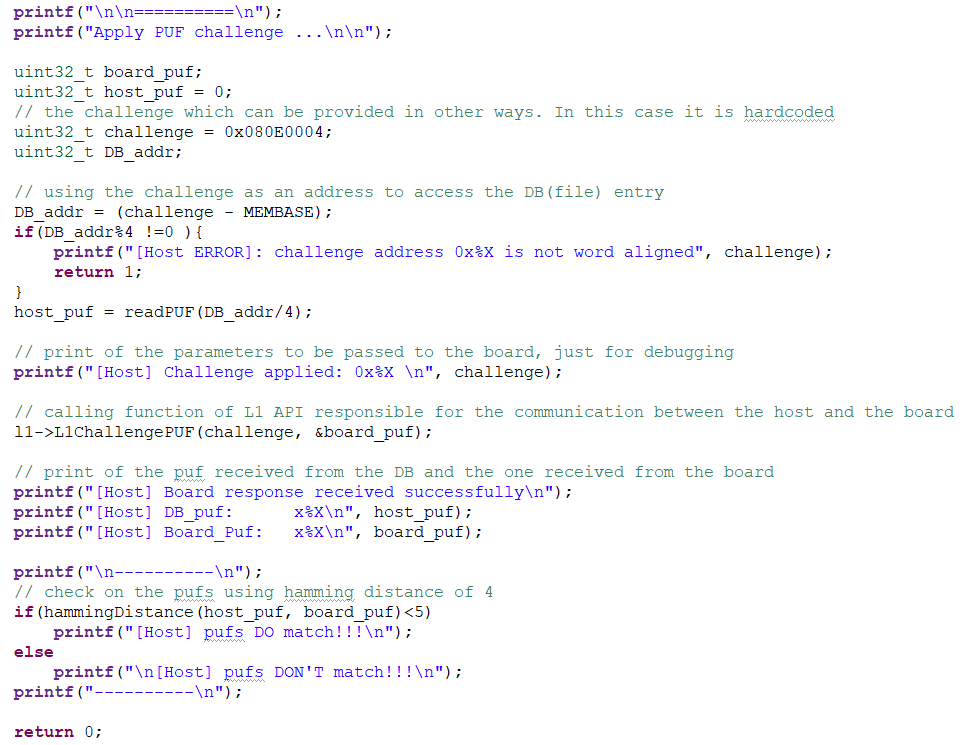
\includegraphics[width = 0.8\textwidth]{images/puf_challenge.png}
	\caption{puf\_challenge.cpp}
	\label{fig:puf_challenge.cpp}
\end{figure}

\subsection{Board side}

The board at this point has been provided with the challenge. However, the data has been sent using little-endian encoding: so, before being able to use the parameter passed, it is necessary to reconstruct the received data to obtain the correct challenge. At this point, the flash memory can be accessed using the challenge as an address. The value at that address will be the actual PUF response to be returned to the host.

\begin{figure}[h!]
	\vspace{0.5cm}
	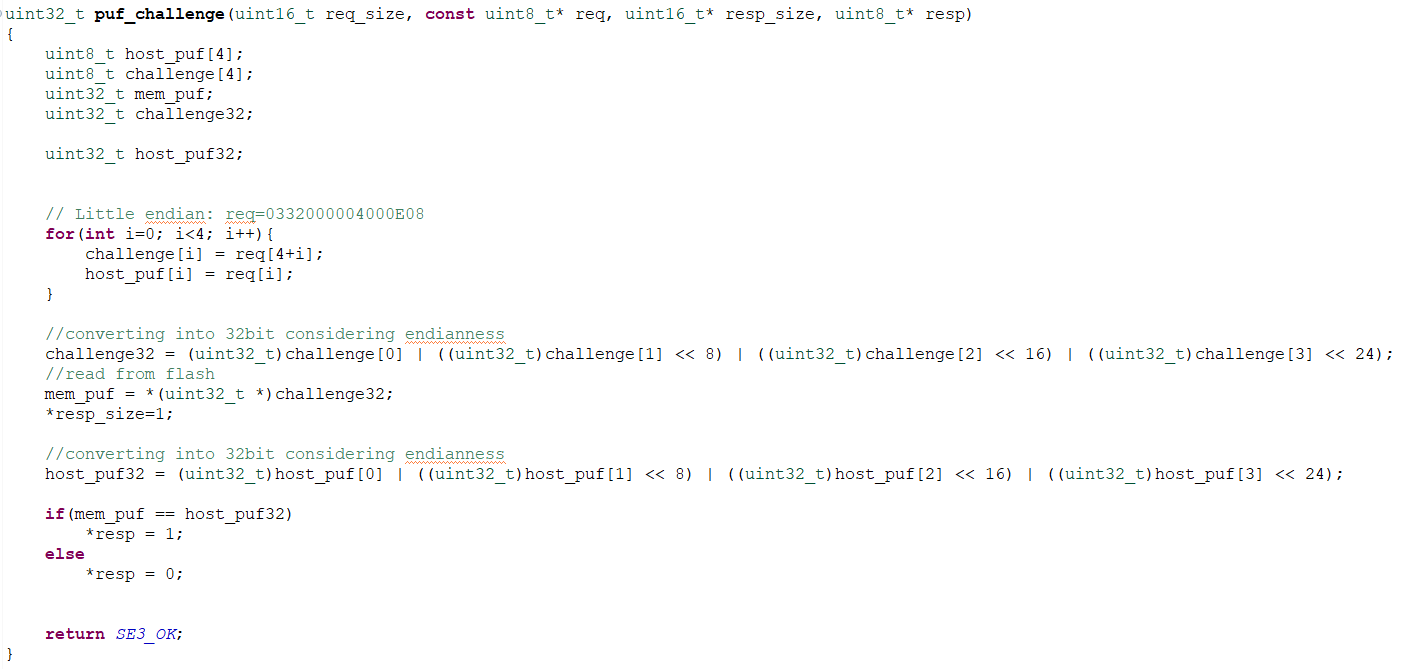
\includegraphics[width = 0.8\textwidth]{images/puf_challenge_board.png}
	\caption{puf\_challenge\_board function on the board side}
	\label{fig:puf_challenge_board}
\end{figure}

The board has now completed its tasks and it is waiting for the next instruction. The host, on the other side, will have to manage the response provided and complete the authentication process.